\documentclass[../SWD_disp.tex]{subfiles}

\begin{document}
\section{Decorator Pattern}
\subsection{Pro}
We use the Decorator pattern to modify an object dynamically. The decorator pattern is used, when we want to use the capabilities of inheritance with sub classes, but add functionality on run time, we want it to be dynamic. We add functionality by using many simple classes, instead of doing it through inheritance. And it is open for extension but not modification. So we want to extend with new code, instead of rewriting old code.
\subsection{Con}
The decorator pattern ends up with a lot of small classes, which increases the complexity. It can also be complicated to have decorators keep track of other decorators. This is because of how the layers are structured. The decorator chain starts to push the pattern besides its actual purpose.

\subsection{Perspektivering}
Chain-of-responsibility pattern
the difference being that for the decorator, all classes handle the request, while for the chain of responsibility, exactly one of the classes in the chain handles the request.

The decorator pattern is structurally nearly identical to the chain of responsibility pattern, the difference being that in a chain of responsibility, exactly one of the classes handles the request, while for the decorator, all classes handle the request.
\subsection{Implementation}


\begin{figure}[H]
    \centering
    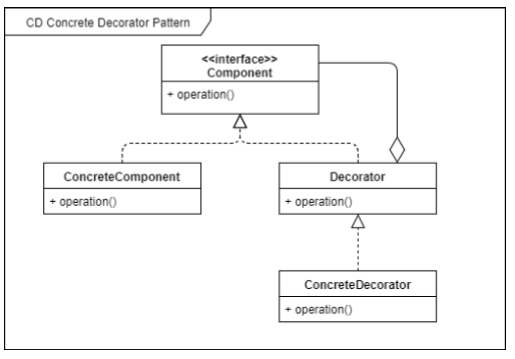
\includegraphics[width = 0.6\textwidth]{decorator_pattern.png}
\end{figure}
\end{document}